\subsection{Типови података}

Осим бројева (целих, у покретном зарезу и других који нису обухваћени јер би иначе обим рада постао превише велики) и променљивих у Python-у постоје и типови података. То су:

\begin{itemize}
\item Ниске (енгл. \emph{strings})
\item Уређене n-торке (енгл. \emph{tuples})
\item Листе (енгл. \emph{lists})
\item Мапе (енгл. \emph{dictionary})
\end{itemize}

Ови типови података могу бити мутабилни (променљиви) и немутабилни (непроменљиви). Тако су листе и речници мутабилни, док су уређене n-торке и ниске непроменљиви. То значи да се, на пример листа која је задата једној променљивој може трајно променити коришћењем наредби и поступака које ће касније бити описане, док рецимо уређене n-торке не могу да се мењају већ само може да се користи њихов садржај.

\subsubsection{Ниске}

Ниска\index{Python!string@стринг} је заправо текст, односно може се размишљати о нисци као секвенци слова. Тако сва слова, бројеви и специјални знаци из овог рада, могу чинити једну ниску. Да би се креирала ниска потребно је поставити низ знакова, тј текст у оквиру наводника. Ниска обично бива додељена некој променљивој.

\begin{lstlisting}[caption = Креирање ниске, label = kreiranje_stringa]
>>> ovo_je_niska = "Hello World!"
\end{lstlisting}
%\pagebreak

Наводници могу бити двоструки и једноструки, резултат ће остати исти. Ако постоји потреба да двоструки или једноструки наводници буду део ниске, ниска ће бити уоквирена једноструким или двоструким наводницима респективно:

\begin{lstlisting}[caption = Примери креирања ниски, label = navodnici]
>>> ovo_je_niska = "Hello World!"
>>> i_ovo_je_niska = 'Hello World!'
>>> i_ovo = 'Kako se kaze "String" na srpskom jeziku?'
>>> moze_i_ovo = "Python je nastao u '90-im godinama proslog veka"
\end{lstlisting}

Приликом приказа на излаз, у ниску могу бити убачени разни динамички или статички подаци који представљају вредност променљиве. Таква радња се обавља помоћу знака \%s у оквиру ниске:

\begin{lstlisting} [caption = Убацивање података у ниску, label = ubacivanje]
>>> moj_prosek = 7.6
>>> poruka = 'Moj prosek je bio %s, a mogao je biti i bolji...'
>>> print (poruka % moj_prosek)
Moj prosek je bio 7.6, a mogao je biti i bolji...
\end{lstlisting}

Будући да је ниска заправо низ знакова, сваки знак има свој редни број у ниски. Први знак је на нултом месту, док се последњем знаку приступа са -1.

\begin{figure}[hеre]
\centering
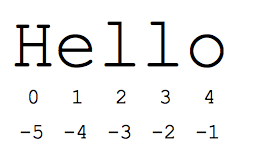
\includegraphics{hello_string.png}
\caption{редни бројеви карактера у ниски}
\label{slike:hello}
\end{figure}


Сад кад је познато како се може приступити појединим знаковима у ниски, могу се набројати које операције са нискама имамо. Постоји више операција са нискама. Табела која следи приказује операције са нискама:

\begin{table}[h]
\centering
\begin{tabular}{|c|c|c|} \hline
\multicolumn{3}{|c|}{\textbf{ОПЕРАЦИЈЕ СА НИСКАМА}}\\ \hline
\textbf{Операције} & \textbf{Објашњење} & \textbf{Пример} \\ \hline
                 + & спајање ниски - конкатенација & s + t \\ \hline
                 * & множење, одн. мултипликација ниски & s * 3 \\ \hline
              s[i] & враћа i-ти знак у ниски & s[-1] \\ \hline
            s[n:m] & враћа све знаке ниске између позиција n и m & s[2:4] \\ \hline
            len(s) & враћа целобројну дужину ниске & len("Hello!") \\ \hline
            str(n) & претвара број у ниску & str(23) \\ \hline
\end{tabular}\medskip
\caption{Операције са нискама}
\label{tabele:strings}
\end{table}

Посебно је интересантна операција исецања ниске (енгл. \emph{slicе}), чиме се даје могућност да се од ниске исече и одвоји тачно онај део који је потребан.

\begin{lstlisting}[caption = Исецање ниске, label = slice]
>>> s = "Hello"         # niska s pokazuje na niz slova Hello
>>> print (s[1:4])      # svi znakovi pocev od drugog zakljucno sa cetvrtim
ell
>>> print (s[1:])       # svi znakovi pocev od drugog do kraja niske
ello
>>> print (s[:])        # svi znakovi od pocetka do kraja
Hello
>>> print (s[1:100])    # svi znakovi pocev od drugog zakljucno sa stotim
ello                    # ako ne postoji 100-i znak, vraca se kraj niske
>>> print (s[-1])       # odredjuje se poslednji znak niske
o
>>> print (s[-4])       # odredjuje se 4. znak od pozadi
e
>>> print (s[:-3])      # svi znaci pocev od pocetka pa do treceg od pozadi
He
>>> print (s[-3:])      # svi znaci pocev od treceg od pozadi do kraja niske
llo

\end{lstlisting}

\subsubsection{Листе}

Листа\index{Python!liste@листе} је мутабилна структура података, у којој се може сачувати секвенца произвољних елемената. Листу могу чинити бројеви, ниске или бројеви и ниске у једној листи. Листа може да садржи друге листе.

Листа се означава помоћу угластих заграда између којих се набрајају чланови листе, одвојени запетом. Ако између две угласте заграде нема ништа, ради се о празној листи. Листа се може мењати, могу се избацивати одговарајући чланови листе, може се променити садржај одговарајућих чланова, а листа се може и допунити новим члановима. Све ове особине чине листе врло корисним оруђем у програмирању.

\begin{lstlisting}[caption = Креирање листе, label = lista]
>>> bitlsi = ['Pol', 'Dzordz', 'Ringo', 'Dzon']
>>> print(bitlsi)
['Pol', 'Dzordz', 'Ringo', 'Dzon']
\end{lstlisting}
%\medskip

\begin{lstlisting}[caption = Креирање празне листе, label = prazna_lista]
>>> prazna_lista = []
>>> print(prazna_lista)
[]
\end{lstlisting}
%\medskip

Кад се креира листа под неким именом, онда то име (променљива) реферише на део меморије у који је уписана дата листа.

\begin{figure}[here]
\centering
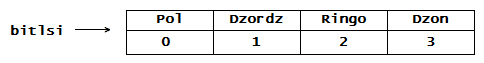
\includegraphics[scale = 0.50]{bitlsi1.png}
\caption{Креирање листе}
\label{slike:lista}
\end{figure}

Ако је потребно да се креира нова листа (на пример \emph{lista}) и њој додели вредност листе \emph{bitlsi}, тада ће и нова листа реферисати на исти меморијски простор. Ако изменимо садржај листе \emph{lista}, аутоматски се мења и садржај листе \emph{bitlsi}.

\begin{figure}[here]
\centering
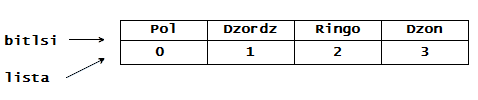
\includegraphics[scale=0.50]{bitlsi2.png}
\caption{lista = bitlsi }
\label{slike:kopiranje}
\end{figure}

На сликама \ref{slike:lista} и \ref{slike:kopiranje}, се може уочити да редни број чланова листе добија вредности на исти начин као и код ниски, дакле: први члан је под редним бројем 0, следећи је 1, итд. Ако је потребно обележити последњи члан листе, користи се редни број -1, претпоследњи је -2, итд.

На листе је могуће применити и исецање листи, на сличан начин како је описано при опису операција са нискама.

\begin{lstlisting}[caption = Исецање листи, label = list_slice][here]
>>> bitlsi = ['Pol', 'Dzordz', 'Ringo', 'Dzon']
>>> print (bitlsi[0:2])
['Pol', 'Dzordz']
>>> print (bitlsi[1])
Dzordz
>>> print (bitlsi[-1])
Dzon
\end{lstlisting}
%\medskip\pagebreak

Оно што највише разликује листе од ниски је способност мутације. Листама се могу додавати или избацивати чланови, листе се могу сортирати. У наредној табели набројане су операције са листама.

\begin{table}[here]\index{Python!operacijesalistama@операције са листама}
\centering
\begin{tabular}{|c|c|c|}\hline
\multicolumn{3}{|c|}{\textbf{ОПЕРАЦИЈЕ СА ЛИСТАМА}}\\ \hline
\textbf{Операције} & \textbf{Објашњење} & \textbf{Пример} \\ \hline
           list[i] & враћа i-ти члан листе & bitlsi[0] \\ \hline
         list[m:n] & даје све чланове почев од m-тог па закључно са n-1 & bitlsi[0:2] \\ \hline
		 len(list) & враћа број чланова листе & len(bitlsi) \\ \hline
		         + & спаја две листе & bitlsi + stonsi \\ \hline
		         * & мултипликује садржај листе & bitlis * 2 \\ \hline
\multicolumn{3}{|c|}{\textbf{МЕТОДЕ}}\\ \hline
    		append & додаје нови члан листе на крај листе & bitlsi.append('Pete')\\ \hline
	    	insert & додаје нови члан на датом месту у листи & bitlsi.insert(1, 'Brian') \\ \hline
		     index & враћа редни број датог члана & bitlsi.index('Pol') \\ \hline
		    remove & брише дати члан листе & bitlsi.remove('Dzon') \\ \hline
		       pop & враћа и брише последњи члан листе & bitlsi.pop() \\ \hline
		      sort & сортира листу & bitlsi.sort() \\ \hline
\end{tabular}
\caption{Операције и методе са листама}
\label{tabela:liste}
\end{table}

\begin{lstlisting}[caption= Мењање листе, label = mutacija_list][here]
>>> bitlsi = ['Pol', 'Dzordz', 'Ringo', 'Dzon']
>>> bitlsi.append('Pit')
>>> print(bitlsi)
['Pol', 'Dzordz', 'Ringo', 'Dzon', 'Pit']
>>> bitlsi.remove('Pit')
>>> print(bitlsi)
['Pol', 'Dzordz', 'Ringo', 'Dzon']
>>> bitlsi.insert(1, 'Pit')
>>> print(bitlsi)
['Pol', 'Pit', 'Dzordz', 'Ringo', 'Dzon']
>>> bitlsi.pop()
'Dzon'
>>> print(bitlsi)
['Pol', 'Pit', 'Dzordz', 'Ringo']
>>> bitlsi.sort()
>>> print(bitlsi)
['Dzordz', 'Pit', 'Pol', 'Ringo']
\end{lstlisting}

Листе су моћно средство програмирања у Python-у, али потребно је бити опрезан кад се употребљавају одговарајуће методе, како се не би јавила грешка (нпр. покушај да се избаци елемент који не постоји у датој листи, доводи до грешке). Такође, треба бити опрезан и код мутирања листе, јер као што је показано ако две променљиве реферишу на исту листу, мењање једне, проузрукује и мењање друге.

\subsubsection{Мапе}\label{subsec:maps}
Мапе\index{Python!mape@мапе} или речници (енгл. \emph{dictionaries}) представљају колекцију елемената, слично као што је то случај и са листама. Разлика између мапа и листа је у томе што се код мапа уместо редних бројева чланова листа, користе парови кључева и њима одговарајућих вредности. Дакле, мапа је структура која се записује тако што се између витичастих заграда набрајају парови који чине један кључ и једна или више вредности везаних за тај кључ. Вредности могу бити бројеви, ниске, листе, уређене n-торке.

\begin{lstlisting}[caption = Разлика између листе и мапе, label = map_vs_list]
>>> bitl_list = [['Pol', 'bas', 'vokal'],
	         ['Dzordz', 'gitara'],
	         ['Ringo', 'bubanj'],
	         ['Dzon', 'gitara', 'vokal']]
>>> print (bitl_list)
[['Pol', 'bas', 'vokal'], ['Dzordz', 'gitara'], ['Ringo', 'bubanj'],
['Dzon', 'gitara', 'vokal']]
>>> bitl_map = {'Pol' : ['bas', 'vokal'],
	        'Dzordz' : ['gitara'],
	        'Ringo' : ['bubanj'],
	        'Dzon' : ['gitara', 'vokal']}
>>> print(bitl_map)
{'Pol': ['bas', 'vokal'], 'Dzordz': ['gitara'],
'Ringo': ['bubanj'], 'Dzon': ['gitara', 'vokal']}
\end{lstlisting}

Ако је потребно да се прикаже шта је Пол свирао, уколико су подаци о групи запамћени као листа, потребно је знати који је Пол редни број у листи, док код мапе редни број не постоји и вредностима се приступа помоћу кључа.

\begin{lstlisting}[caption = Кључ и вредност, label = key_value]
>>> print (bitl_map['Pol'])
['bas', 'vokal']
\end{lstlisting}

Ако је задатак да се утврди ко је све свирао гитару у Битлсима, потребно је испитати сваки елемент листе. Тај задатак ће бити решаван у поглављима која следе, када се буду обрађивале теме везане за петље и модуле.

Због природе мапа, мутација је прилично другачија у односу на листе. Да би се додао нови елемент, односно пар кључ-вредност, потребно је уз име мапе ставити нови кључ и доделити му вредност или изменити постојећу. Такође помоћу команде \emph{del}, могуће је обрисати кључ, а тиме и вредност везану за њега.

\begin{lstlisting}[caption = Мутација мапа, label = mutacija_mapa]
>>> bitl_map['Pit']='bubanj'
>>> bitl_map['Dzordz']=['gitara', 'vokal'] # dodan je vokal Dzordzu
>>> del bitl_map['Pit']
\end{lstlisting}

Могуће је креирати и празну мапу, једноставно се остави празан простор између две витичасте заграде.

\begin{lstlisting}[caption = Креирање празне мапе, label=prazna_mapa]
>>> prazna_mapa = {}
\end{lstlisting}

Методи и функције за рад са мапама су различити у односу на листе, јер не постоје, на пример \emph{pop} и \emph{append} методе који омогућавају мутацију, већ да би се мењала мапа потребно је знати који елемент се убацује, мења или избацује из дате мапе.

\begin{table}[here]
\centering
\begin{tabular}{|c|c|c|} \hline
\multicolumn{3}{|c|}{\textbf{МЕТОДИ И ФУНКЦИЈЕ ЗА РАД СА МАПАМА}} \\ \hline
\textbf{Метода} & \textbf{Објашњење} & \textbf{Пример} \\ \hline
map[key]=value & Додељивање или мењање вредности кључа & bitlsi['Dzon'] = 'vokal' \\ \hline
del map[kljuc] & Брисање кључа и вредности из мапе & del bitlsi['Pol'] \\ \hline
keys() & Метод којим се сви кључеви дате мапе враћају као листа & bitlsi.keys() \\ \hline
values() & Метод којим се све вредности дате мапе враћају као листа & bitlsi.values() \\ \hline
items() & Метод који враћа листу уређених парова кључ, вредност & bitlsi.items() \\ \hline
\end{tabular}
\caption{Методе и функције за рад са мапама}
\label{tabela:mape}
\end{table}

\subsubsection{Уређене n-торке}

У Python-у постоји начин да подаци сместе у уређене n-торке\index{Python!tapl@тапл}, где $n \in \mathbb{N}\cup\{0\}$. Подаци се смештају између две заграде и раздвојени су зарезом. Python интерпретатору није потребно да их ставимо између заграда, док год су подаци раздвојени зарезом, већ ће он свако набрајање схватити као уређену n-торку, чак и ако нема заграде.

\begin{lstlisting} [caption = Креирање уређене n-торке, label = tuple]
>>> fibo = (0, 1, 1, 2, 3)
>>> print (fibo)
(0, 1, 1, 2, 3)

>>> fibo1 =0, 1, 1, 2, 3  # uredjena n-torka bez zagrada
>>> print (fibo1)
(0, 1, 1, 2, 3)

>>> prazan = () # kreiranje prazne uredjene n-torke
>>> print (prazan)
()

>>> jedan_clan = (1,) # jednoclana uredjena n-torka mora imati
>>> print (jedan_clan) # zarez, iako ne postoji drugi broj
(1,)
\end{lstlisting}
%\pagebreak

У уређеним n-торкама је могуће сместити вредности и других типова података, као што су бројеви и ниске. Такође, могуће је сместити и листе и друге уређене n-торке, док год се поштује горе наведена синтакса.

\begin{lstlisting}[caption = Уређене n-торке могу садржати и ниске и  листе и друге уређене n-торке, label = str_lst_tuple]
>>> niska = ('a', 'b')
>>> print (niska)
('a', 'b')
>>> lst = ([1, 2, 3], [1,2])
>>> print (lst)
([1, 2, 3], [1, 2])
>>> tapl = ((1,), (), (1, 2, 3))
>>> print (tapl)
((1,), (), (1, 2, 3))
\end{lstlisting}

Оно што највише разликује уређене n-торке од осталих типова података је да су они у потпуности непроменљиви. Када се креира уређена n-торка, могуће је искључиво користити њене вредности, док је немогуће мењати или додавати вредности уређених n-торки. Могуће је, уколико се за тим укаже потреба доћи  до појединих чланова уређених n-торки, ако се зна њихов редни број, а могуће је исецати уређене n-торке, слично као код ниски.
